\section{Adaptive Kriging}\label{sec:AK_PF}

In this section, we propose to use training data subsampling, \textit{i.e.} selecting a subset $\tilde{\mathbf{x}}^r$ of $\tilde{N}^r$ training points and using only these points for regression, as a way to alleviate the computational issues raised above. Since the computational and memory costs of kriging scale quadratically with the number of training points, discarding half the data reduces the computational load by a factor of $4$ and requires $4$ times less storage.

However, this method comes at a cost. In the following, we describe two subsampling strategies, each requiring to perform a subsampling step at each time step. This means that no precomputation can be done before the mission, and in particular that inverting $G(\tilde{\mathbf{x}}^r)\in\mathcal{S}_{\tilde{N}^r\:d_z}^{++}(\mathbb{R})$ and $C^\top G(\tilde{\mathbf{x}}^r)^{-1}C\in\mathcal{S}_{d_z}^{++}(\mathbb{R})$ must be done online.

\subsection{Random Subsampling}

The simplest idea to reduce the number of training points is to let $p\in[0,1]$, and draw independently $s_{i,k}$ from a Bernoulli distribution of success probability $p$, for each $i\in[\![1,\tilde{N}]\!]$. Any training sample $\tilde{x}_i$ for which the corresponding $s_{i,k}$ is a success is retained to form $\tilde{\mathbf{x}}_{\mathrm{RS},k}^r$, while the others are discarded. This operation is performed at the beginning of each time step to avoid skewing the reconstruction. Since the training points are randomly selected across the map rather than localised to a specific region of space, the hyperparameters are estimated before the mission on the entire training set, similarly to the static kriging version.

By linearity of the expectation, the number of retained data is, on average:
\begin{equation}
	\mathbb{E}\left[\tilde{N}_{\mathrm{RS},k}^r\right]=p\:\tilde{N}
\end{equation}
and corresponds, on average, to the density of a regular grid of resolution $\Delta_g/\sqrt{p}$.

Similarly to the case of bilinear interpolation and static kriging presented above, the simulations described in \Cref{sec:scenario} were run using random subsampling with:
\begin{equation}
	p=0.5
\end{equation}

The results are compared here with those obtained with static kriging. \Cref{fig:eclairci_RMSE,fig:eclairci_NEES} respectively compare the RMSE and NEES of the two approaches on each of the six grid resolutions, while \Cref{fig:convergence_eclairci} presents the corresponding convergence rates. Finally, \Cref{tab:cout_eclairci} gives the comparative computational cost of each method across the six resolutions.

\begin{figure}[!p]
	\centering
	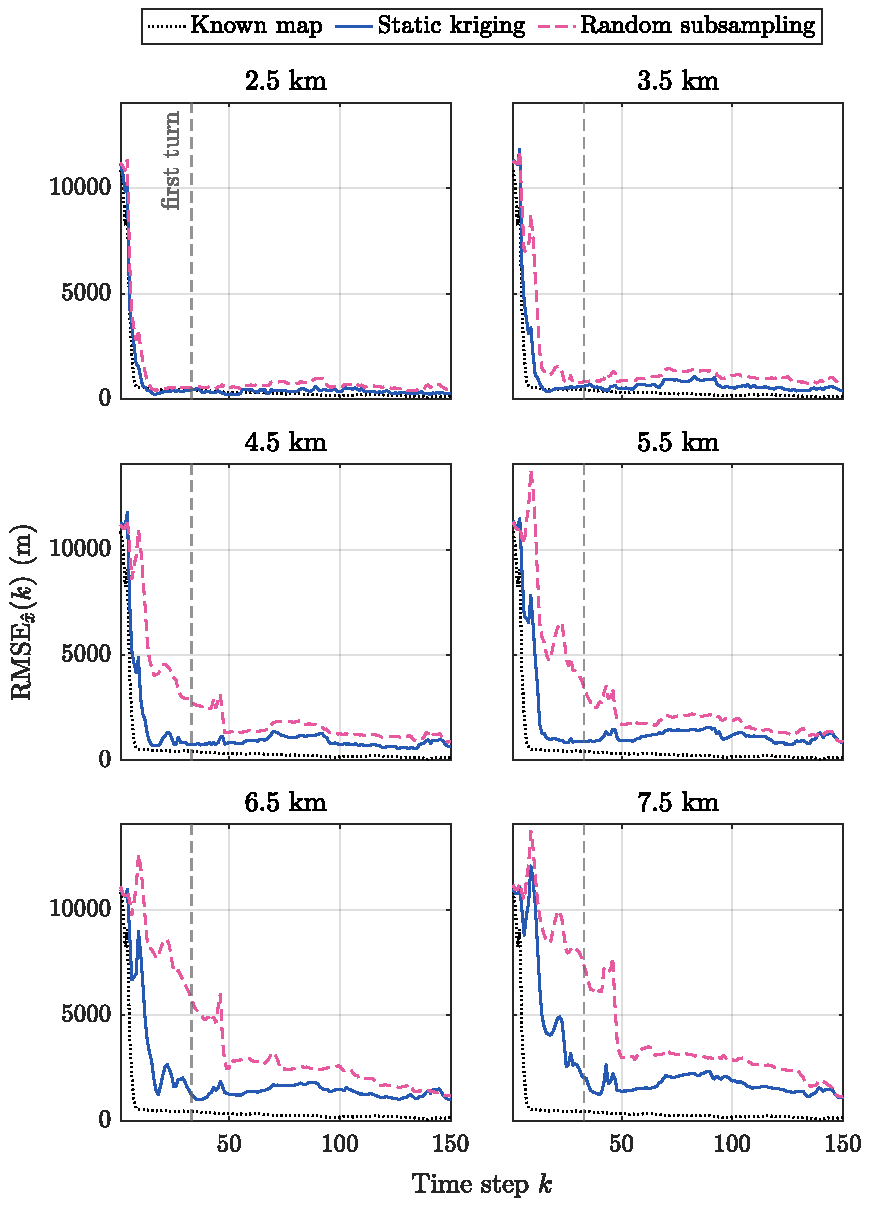
\includegraphics[width=\textwidth]{../../Images/RMSE eclairci par maille.pdf}
	\caption{Comparative RMSE of the navigation algorithms using static kriging or random subsampling across the six grid resolutions. The performance of the filter with access to the true map is given as a reference.}\label{fig:eclairci_RMSE}
\end{figure}

\begin{figure}[!p]
	\centering
	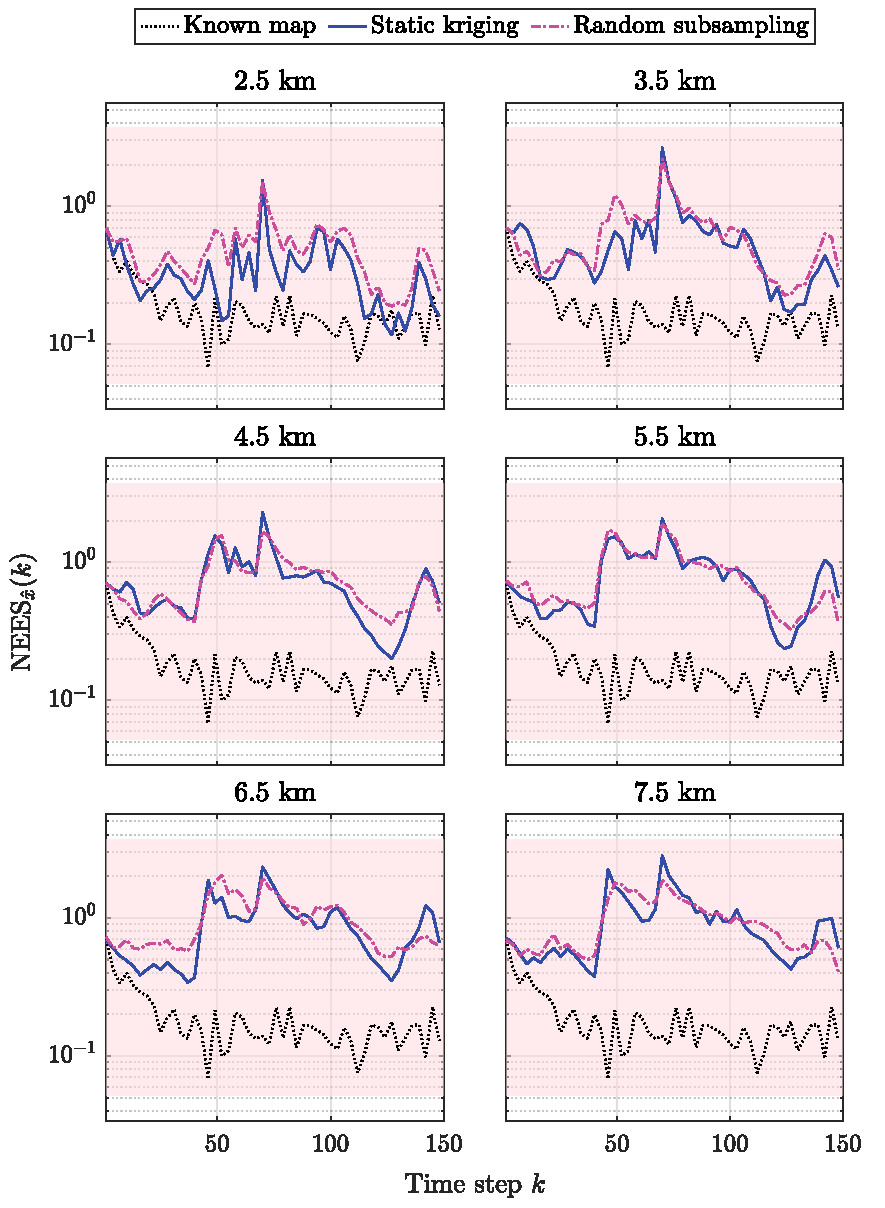
\includegraphics[width=\textwidth]{../../Images/NEES eclairci par maille.pdf}
	\caption{Comparative RMSE of the navigation algorithms using static kriging or random subsampling across the six grid resolutions. The shaded area corresponds to that of the previous NEES figure.}\label{fig:eclairci_NEES}
\end{figure}

\begin{figure}[!htb]
	\centering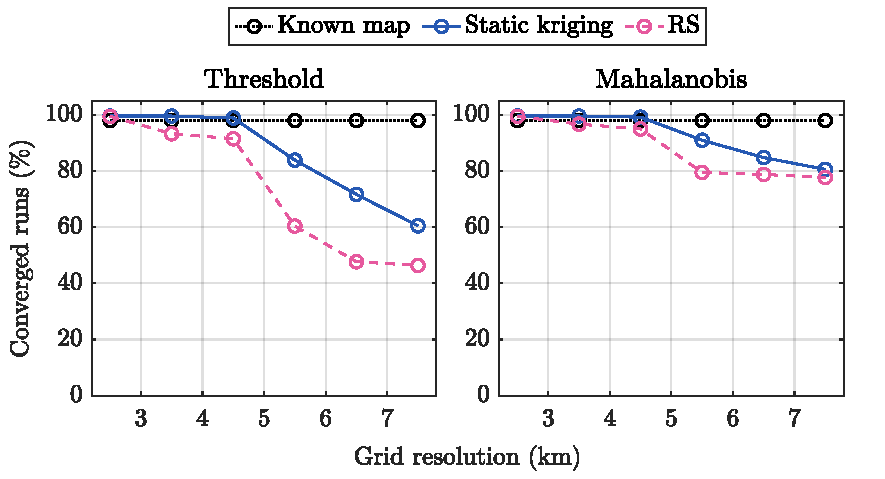
\includegraphics[width=\textwidth]{../../Images/Convergence eclairci.pdf}
	\caption{Convergence rates for the navigation algorithms using static kriging and random subsampling as a function of grid resolution.}\label{fig:convergence_eclairci}
\end{figure}

\begin{table}[!htb]
	\centering% Generated by figures_campagnes.m, do not edit by hand.
% Static kriging against RS.
% Analytic flop counts per run, not timings, for 5000 particles over 150 steps.
% The kriging column gathers the factorisation and the queries, which no
% method pays one without the other; the hyperparameter column is the local
% fits, and the last column, where there is one, the mean-shift of the ICAK and
% the MCAK, or
% the neighbour search of the NNAK. A method that does not pay a cost has no
% column for it.
% Where the training set is fixed, n^3/3 for the setup plus N n^2 per query.

\begin{tabular}{|c|c|c|}\hline
$\Delta_g$ & Static kriging & RS\\\hline
$2.5$ km & $29.3$ T & $7.3$ T\\
$3.5$ km & $7.39$ T & $1.84$ T\\
$4.5$ km & $2.81$ T & $704$ G\\
$5.5$ km & $1.26$ T & $314$ G\\
$6.5$ km & $608$ G & $152$ G\\
$7.5$ km & $343$ G & $85.9$ G\\
\hline
\end{tabular}

	\caption{Total computational cost, in flops, of using static kriging or random subsampling throughout the mission, for each grid resolution.}\label{tab:cout_eclairci}
\end{table}

For the RMSE curves, random subsampling is systematically outperformed by static kriging, especially before the first turn. From $4.5$ km onward, random subsampling only reaches its error plateau during this turn, whereas static kriging stabilises before it. This indicates that, although the subsampling (RS) is randomised at each time step, and each training point is therefore available to the filter on average $50\%$ of the time, the resulting map is too degraded to provide an accurate navigation solution. The late convergence of the filters with access to the fewest training points is likely a consequence of the additional information provided by the first turn.

Nevertheless, the similarity between random subsampling at $\Delta_g=2.5$ and $5.5$ km and static kriging at $\Delta_g=3.5\approx2.5/\sqrt{0.5}$ and $7.5\approx5.5/\sqrt{0.5}$ km respectively, is noteworthy. This suggests that random subsampling effectively behaves as a map with a degraded resolution. Although the full training set is likely to have been sampled at least once over the course of the mission, only half of the points are available to the filter at each time step.

Regarding the NEES, the curves are consistently similar between both methods, further highlighting the ability of kriging to accurately quantify its uncertainty. As already established in \Cref{sec:kriging_method}, the kriging covariance increases in regions where less data are available, and thus the predicted uncertainty naturally follows the degradation of the map. Despite this, random subsampling achieves lower convergence rates at every grid resolution, showing that this method is unable to match the navigation performance of static kriging.

Finally, \Cref{tab:cout_eclairci} illustrates the only advantage of random subsampling over static kriging. By reducing the number of available training points by half on average, this method reduces the computational cost by approximately $75\%$ at every grid resolution.

\subsection{Adaptive Subsampling Window}\label{sec:AK}

The above results show that, while subsampling does reduce the computational cost of the algorithm, indiscriminately discarding training points is detrimental to the navigation performance. A more suitable strategy should therefore retain only a limited number of training points while selecting those that are most relevant to the current situation.

Since, at each time step, the filter only queries the map where its particles lie, this suggests retaining the points surrounding the particle set. Beyond reducing the computational cost, a local selection also relaxes a second limitation of static kriging. Indeed, the estimators introduced in \cref{sec:kriging} assume the use of a single kernel over the entire domain, and \cref{th:kriging_navigation_assumptions} inherits that hypothesis. In \cref{sec:HP_estimation}, we estimated the hyperparameters of the kernel once before the mission, meaning that they are assumed to be independent of the inputs:
\begin{equation}
	k_{3/2}:x,x'\mapsto\sigma_f^2\left(1+\frac{\sqrt{3}\:\|x-x'\|_2}{l}\right)\exp\left(-\frac{\sqrt{3}\:\|x-x'\|_2}{l}\right)
\end{equation}

The considered kernel is thus radial, and the resulting GP is therefore stationary. This is unrealistic for a physical field, especially at large spatial scales. However, stationarity cannot be simply dropped, as the hyperparameters of such a kernel would have to be fitted at every point of the domain, where a single sample is available. We therefore assume the field to be non-stationary, but its hyperparameters to vary over a scale much larger than the grid resolution of the training data. Under this hypothesis, the hyperparameters must be estimated over a region large enough to provide sufficient data for accurate estimation, while remaining small enough to avoid averaging them over distances on which they vary significantly.

In this section, we propose an adaptive subsampling strategy to optimise the kriging performance of the filter according to four criteria:
\begin{itemize}
	\item The retained training points must cover an area large enough to avoid extrapolation at the particle locations.
	\item A sufficient number of training points must be considered to ensure that the hyperparameters are accurately estimated.
	\item The retained training points must be confined to a sufficiently small region for the hyperparameters to be approximately constant within this region.
	\item Finally, their number must remain small enough to ensure that the filter can be computed within real-time constraints.
\end{itemize}

The first constraint naturally gives the shape of the retained subset. Let $\hat{x}_{k|k-1}$ be the predicted estimate of the filter at time $k$:
\begin{equation}
	\hat{x}_{k|k-1}\triangleq\sum_{i=1}^Nw_{k-1}^{(i)}\:x_k^{(i)}\approx\mathbb{E}_{p(\cdot|\mathbf{z}_{1:k-1})}[x_k]
\end{equation}
and $\hat{P}_{k|k-1}$ denote the corresponding covariance matrix:
\begin{equation}
	\hat{P}_{k|k-1}\triangleq\sum_{i=1}^Nw_{k-1}^{(i)}\left(x_k^{(i)}-\hat{x}_{k|k-1}\right)\left(x_k^{(i)}-\hat{x}_{k|k-1}\right)^\top
\end{equation}

These two quantities can be computed after the prediction step at time $k$, but before the following weight update, and represent a Gaussian approximation of the particle set at time $k$ before kriging the environment. It must be noted that, while the selection itself should only depend on the particle locations, both sums are weighted by the $w_{k-1}^{(i)}$ to limit the effect of resampling on the resulting moments. Although this may result in some particles being left outside the retained region, this is not detrimental when their associated weights are low.

In this approximation, each particle has a $99\%$ chance to verify:
\begin{equation}
	\left\|\Pi_{\mathrm{pos}}\:\hat{x}_{k|k-1}-\Pi_{\mathrm{pos}}\:x_k^{(i)}\right\|_{\hat{P}_{\mathrm{pos},k|k-1}}^2\leq\chi_{d_{\mathrm{pos}}}^2(99\%)
\end{equation}
where $d_{\mathrm{pos}}$ is the dimension of the position subspace, $\hat{P}_{\mathrm{pos},k|k-1}$ is the covariance matrix associated with the projection of the predicted state onto this subspace:
\begin{equation}
	\hat{P}_{\mathrm{pos},k|k-1}\triangleq\Pi_{\mathrm{pos}}\:\hat{P}_{k|k-1}\:\Pi_{\mathrm{pos}}^\top
\end{equation}
and $\chi_{d_{\mathrm{pos}}}^2(99\%)$ is the $99\%$ quantile of a $\chi^2$ distribution with $d_{\mathrm{pos}}$ degrees of freedom. This means that the particles are likely to be contained in an ellipsoid centred on $\Pi_{\mathrm{pos}}\:\hat{x}_{k|k-1}$, and whose shape is given by the eigenvectors of $\hat{P}_{\mathrm{pos},k|k-1}$.

However, this geometry is tied to the particle set, and does not directly translate into the physical position space. Furthermore, when $\hat{P}_{\mathrm{pos},k|k-1}$ is highly anisotropic, the resulting ellipsoid may provide insufficient coverage along directions of lower uncertainty, leading to extrapolation. To solve this issue, we use the Rayleigh quotient \cite{bib:matrix-cookbook} to convert the Mahalanobis inequality into a Euclidean one:
\begin{equation}
	\begin{aligned}
	\left\|\Pi_{\mathrm{pos}}\:\hat{x}_{k|k-1}-\Pi_{\mathrm{pos}}\:x_k^{(i)}\right\|_2^2&\leq\lambda_{\max}\left(\hat{P}_{\mathrm{pos},k|k-1}\right)\left\|\Pi_{\mathrm{pos}}\:\hat{x}_{k|k-1}-\Pi_{\mathrm{pos}}\:x_k^{(i)}\right\|_{\hat{P}_{\mathrm{pos},k|k-1}}^2\\
	&\leq\chi_{d_{\mathrm{pos}}}^2(99\%)\:\lambda_{\max}\left(\hat{P}_{\mathrm{pos},k|k-1}\right)
	\end{aligned}
\end{equation}

The first subsampling criterion is thus satisfied by retaining training points within a ball of radius:
\begin{equation}
	r_{\mathrm{cov},k}\triangleq\alpha_{\mathrm{cov}}\sqrt{\chi_{d_{\mathrm{pos}}}^2(99\%)}\sqrt{\lambda_{\max}\left(\hat{P}_{\mathrm{pos},k|k-1}\right)}\label{eq:r_cov}
\end{equation}
and centred on $\Pi_{\mathrm{pos}}\:\hat{x}_{k|k-1}$, where $\alpha_{\mathrm{cov}}\geq1$ is a dilation factor, introduced to provide a margin around the particle set and reduce the risk of extrapolation at its boundaries.

However, when the particle set collapses on a small region of space, the ball may not contain enough training points to satisfy the second criterion. We thus introduce a second radius to ensure that at least $\tilde{N}_{\min}$ training points are retained:
\begin{equation}
	r_{\min,k}\triangleq\min_{r\in\mathbb{R}^+}\left(\operatorname{Card}\left\{i\in[\![1,\tilde{N}]\!]\:\middle|\:\left\|\Pi_{\mathrm{pos}}\:\hat{x}_{k|k-1}-\tilde{x}_i\right\|_2\leq r\right\}\geq\tilde{N}_{\min}\right)\label{eq:r_min}
\end{equation}

The retained training set is thus defined at each time step $k$ as:
\begin{equation}
	\tilde{\mathbf{x}}_{\mathrm{AK},k}^r\triangleq\left\{\tilde{x}_i\in\tilde{\mathbf{x}}\:\middle|\:\left\|\Pi_{\mathrm{pos}}\:\hat{x}_{k|k-1}-\tilde{x}_i\right\|_2\leq\max\left(r_{\mathrm{cov},k},r_{\min,k}\right)\right\}\label{eq:AK_window}
\end{equation}
and:
\begin{equation}
	\tilde{\mathbf{z}}_{\mathrm{AK},k}^r\triangleq\{\tilde{z}_i\mid\tilde{x}_i\in\tilde{\mathbf{x}}_{\mathrm{AK},k}^r\}\label{eq:AK_window_z}
\end{equation}

At each time step, the hyperparameters $\hat{\theta}_k$ of the kernel are then re-estimated by maximum likelihood on the retained training set, as described in \cref{sec:HP_estimation}. In particular, since the navigation estimate varies slowly between two consecutive time steps, the latter is likely to remain similar. The hyperparameters estimated at time $k-1$ can thus be used as initial values for the estimation at time $k$, reducing the number of iterations required for convergence of the hyperparameter estimation algorithm.

In particular, the number of retained points is, on average, the $d_{\mathrm{pos}}$-volume of the window divided by that of a grid cell:
\begin{equation}
	\mathbb{E}\left[\tilde{N}_{\mathrm{AK},k}^r\right]=\frac{\pi^{d_{\mathrm{pos}}/2}}{\Gamma\left(\frac{d_{\mathrm{pos}}}{2}+1\right)}\left(\frac{\max\left(r_{\mathrm{cov},k},r_{\min,k}\right)}{\Delta_g}\right)^{d_{\mathrm{pos}}}\label{eq:AK_window_size}
\end{equation}

The likelihood \eqref{eq:kriged_likelihood} is thus computed on the retained subset alone and using the updated hyperparameters:
\begin{equation}
	z_k|x_k,\tilde{\mathbf{z}}_{\mathrm{AK},k}^r\sim\mathcal{N}\left(\hat{z}_{\mathrm{OK}}\left(x_k,\tilde{\mathbf{x}}_{\mathrm{AK},k}^r,\tilde{\mathbf{z}}_{\mathrm{AK},k}^r;\hat{\theta}_k\right),R_{\mathrm{OK}}\left(x_k,\tilde{\mathbf{x}}_{\mathrm{AK},k}^r;\hat{\theta}_k\right)\right)\label{eq:AK_likelihood}
\end{equation}

This method, referred to as Adaptive Kriging (AK) and originally proposed in \cite{bib:AK-PF}, can be integrated into any navigation algorithm presented in \cref{sec:Bayesian_estimation}. In this section, we focus on its integration into the RPF of \Cref{alg:RPF} using the transition density as proposal, as described in \eqref{eq:prior_proposal}. The resulting algorithm is the Adaptive Kriging Regularised Particle Filter (AK-RPF) given in \Cref{alg:AK_RPF}.

\begin{algorithm}[!htb]
	\begin{algorithmic}
	\State{$\forall i\in[\![1,N]\!],\:x_k^{(i)}\sim p\left(\cdot|x_{k-1}^{(i)}\right)$}\Comment{Particle propagation}
	\State{$\displaystyle\hat{x}_{k|k-1}=\sum_{i=1}^Nw_{k-1}^{(i)}x_k^{(i)}$}\Comment{\textbf{Predicted estimation}}
	\State{$\displaystyle\hat{P}_{k|k-1}=\sum_{i=1}^Nw_{k-1}^{(i)}\left(x_k^{(i)}-\hat{x}_{k|k-1}\right)\left(x_k^{(i)}-\hat{x}_{k|k-1}\right)^\top$}
	\State{Compute $\tilde{\mathbf{x}}_{\mathrm{AK},k}^r$ with \eqref{eq:AK_window}}\Comment{\textbf{Adaptive subsampling}}
	\State{Compute $\tilde{\mathbf{z}}_{\mathrm{AK},k}^r$ with \eqref{eq:AK_window_z}}
	\State{$\hat{\theta}_k=\operatorname{MLE}\left(\tilde{\mathbf{x}}_{\mathrm{AK},k}^r,\tilde{\mathbf{z}}_{\mathrm{AK},k}^r,\hat{\theta}_{k-1}\right)$}\Comment{\textbf{Hyperparameter estimation}}
	\State{$\forall i\in[\![1,N]\!],\:$compute $\tilde{p}\left(z_k|x_k^{(i)}\right)$ from \eqref{eq:AK_likelihood}}\Comment{\textbf{Kriging}}
	\State{$\forall i\in[\![1,N]\!],\:\tilde{w}_k^{(i)}=w_{k-1}^{(i)}\:\tilde{p}\left(z_k|x_k^{(i)}\right)$}\Comment{Weight update}
	\State{$\displaystyle\forall i\in[\![1,N]\!],\:w_k^{(i)}=\left.\tilde{w}_k^{(i)}\middle/\sum_{j=1}^N\tilde{w}_k^{(j)}\right.$}\Comment{Normalisation}
	\State{$\displaystyle\hat{N}_{\mathrm{eff}}=\left.1\middle/\sum_{i=1}^N\left(w_k^{(i)}\right)^2\right.$}\Comment{Resampling criterion}
	\If{$\hat{N}_{\mathrm{eff}}<N_{\mathrm{th}}$}
	\State{$\displaystyle\hat{x}_k=\sum_{i=1}^Nw_k^{(i)}x_k^{(i)}$}\Comment{Whitening}
	\State{$\displaystyle\hat{P}_k=\sum_{i=1}^Nw_k^{(i)}\left(x_k^{(i)}-\hat{x}_k\right)\left(x_k^{(i)}-\hat{x}_k\right)^\top$}
	\State{$A_k\text{ s.t. }\hat{P}_k=A_k\:A_k^\top$}
	\State{$\left\{x_k^{(j)},w_k^{(j)},-\right\}_{j=1}^N\gets\operatorname{Resampling}\left(\left\{x_k^{(i)},w_k^{(i)}\right\}_{i=1}^N\right)$}\Comment{Resampling}
	\State{$\forall j\in[\![1,N]\!],\:\varepsilon^{(j)}\sim K$}\Comment{Regularisation}
	\State{$\forall j\in[\![1,N]\!],\:x_k^{(j)}\gets x_k^{(j)}+\alpha_{\mathrm{reg}}hA_k\:\varepsilon^{(j)}$}
	\EndIf
	\end{algorithmic}\caption{Adaptive Kriging Regularised Particle Filter}\label{alg:AK_RPF}
\end{algorithm}

Unfortunately, the third and fourth criteria may conflict with the first one in situations where the particle set spans over a large region of space. These two criteria are addressed in \cref{sec:window_shape}.

\subsection{Numerical Results}

As for static kriging, this section evaluates the performance of the AK-RPF across the six grid resolutions, with:
\begin{equation}
\alpha_{\mathrm{cov}}=2\quad\text{and}\quad\tilde{N}_{\min}=25
\end{equation}

The performance of the static kriging RPF is also given as a reference. Alongside the RMSE and the NEES, another metric is introduced to help explain the variations in computational cost between each configuration. This metric is the number of retained training points, \textit{i.e.} the value of $\tilde{N}^r$, at each time step. \Cref{fig:AK_RMSE,fig:AK_NEES} present the comparative RMSE and NEES curves across the six grid resolutions, and \Cref{fig:convergence_AK} gives the associated convergence rates. Finally, \Cref{fig:AK_echantillons} shows the evolution of the average number of retained training points throughout the mission, and \Cref{tab:cout_adaptatif} presents the average total computational cost of static kriging and AK during the entire mission for each of the six grid resolutions.

\begin{figure}[!p]
	\centering
	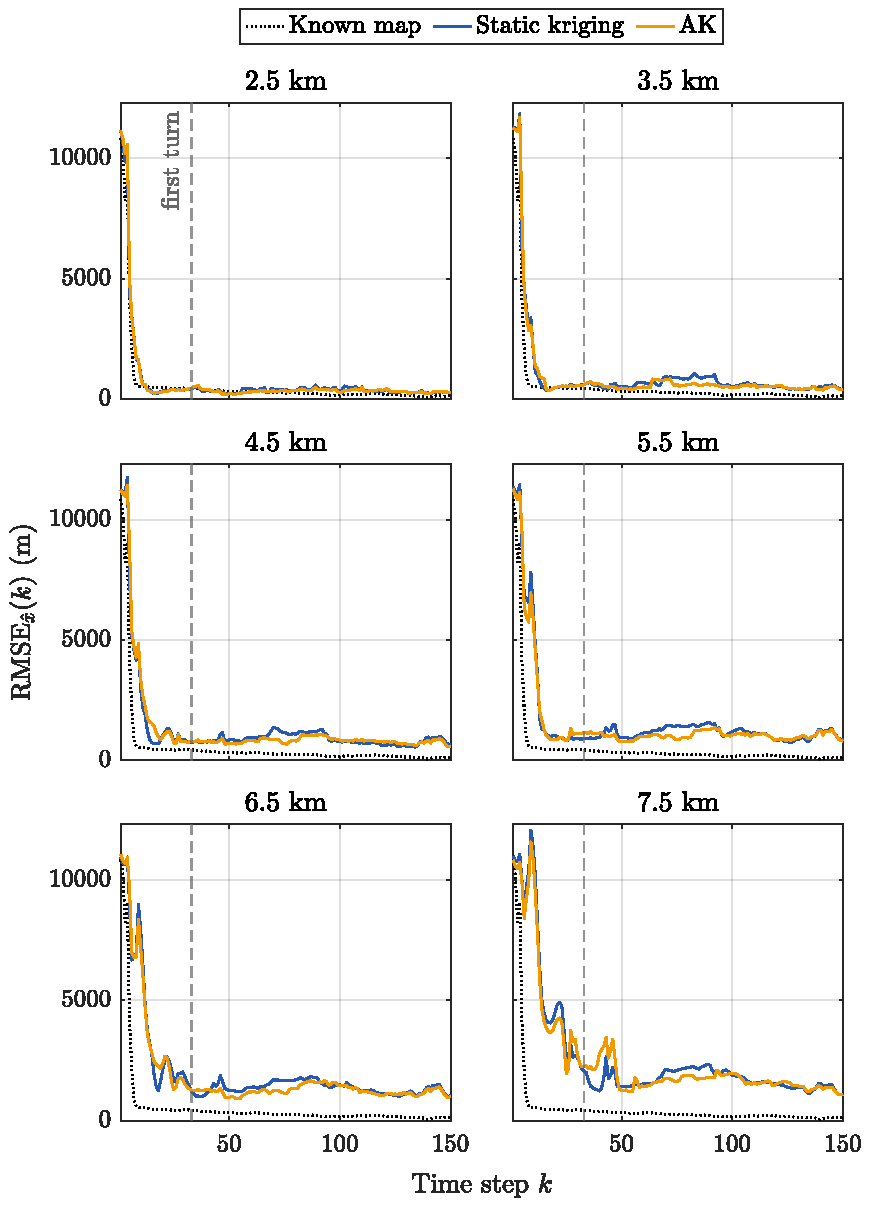
\includegraphics[width=\textwidth]{../../Images/RMSE adaptatif par maille.pdf}
	\caption{RMSE curves for the AK-RPF compared with that of an RPF using static kriging acorss the six grid resolutions.}\label{fig:AK_RMSE}
\end{figure}

\begin{figure}[!p]
	\centering
	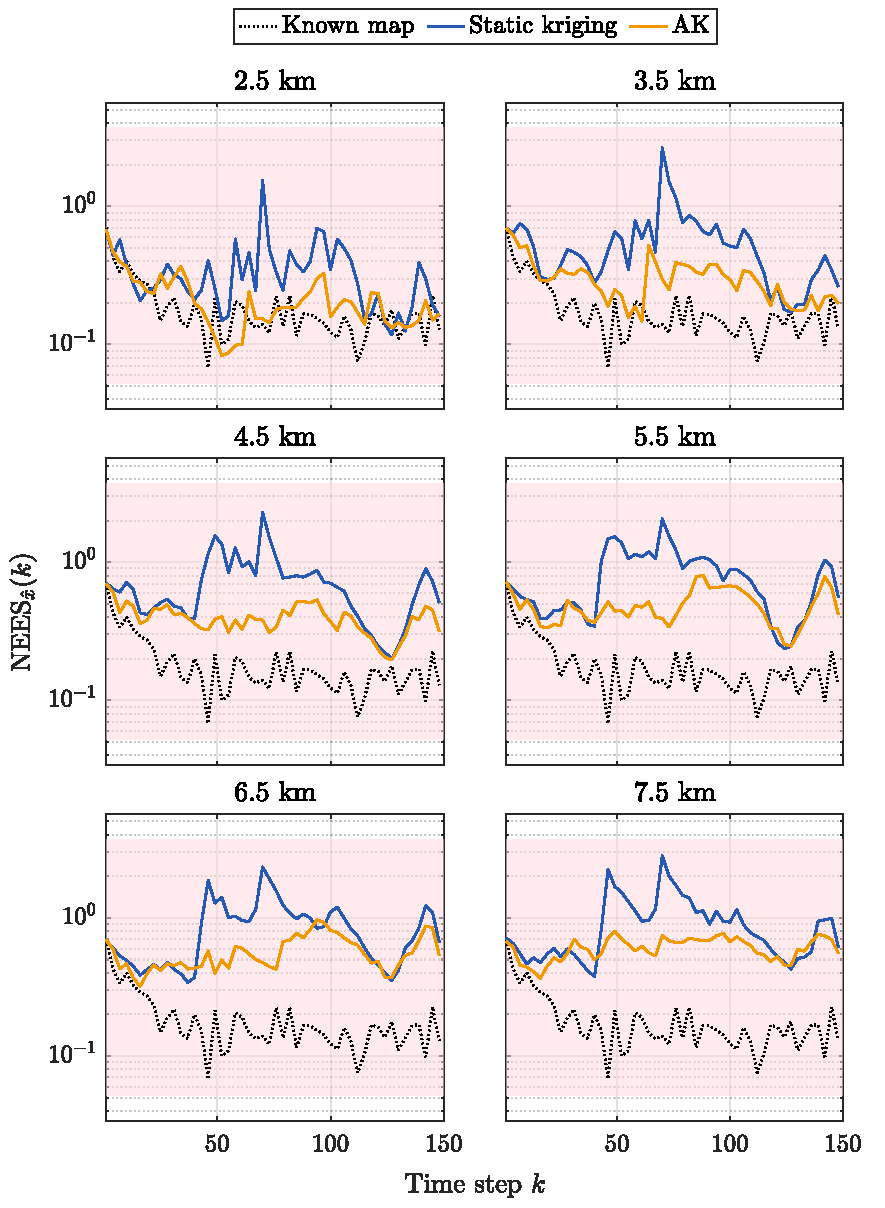
\includegraphics[width=\textwidth]{../../Images/NEES adaptatif par maille.pdf}
	\caption{NEES curves for the AK-RPF compared with that of an RPF using static kriging acorss the six grid resolutions.}\label{fig:AK_NEES}
\end{figure}

\begin{figure}[!htb]
	\centering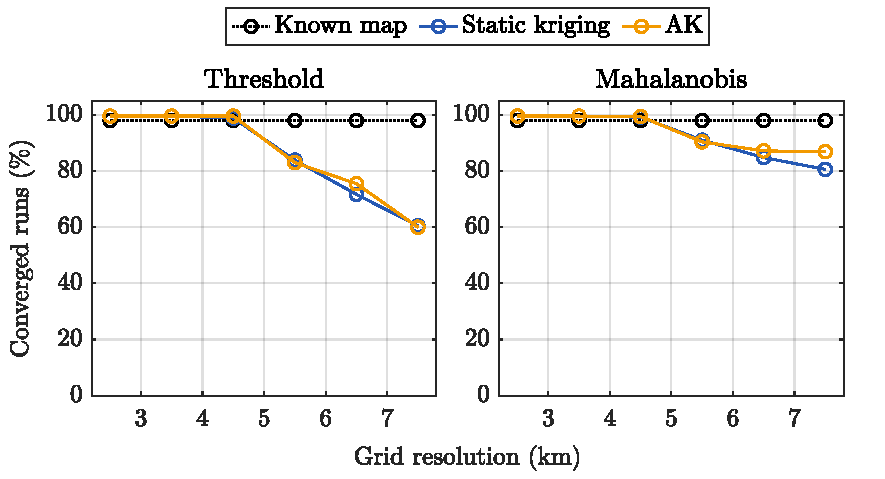
\includegraphics[width=\textwidth]{../../Images/Convergence adaptatif.pdf}
	\caption{Convergence rates of the AK-RPF and the RPF using static kriging using the threshold and the Mahalanobis criteria.}\label{fig:convergence_AK}
\end{figure}

\begin{figure}[!htb]
	\centering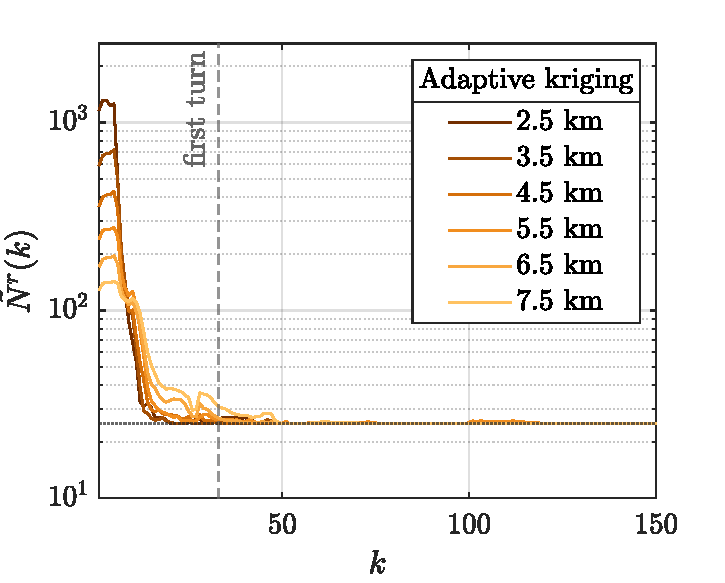
\includegraphics[width=\textwidth]{../../Images/Echantillons retenus par maille.pdf}
	\caption{Evolution of the average number of training points retained by the AK-RPF during the mission for each grid resolution. A logarithmic scale is used before the first turn at $k=33$ to capture the large variations in $\tilde{N}^r_{\mathrm{AK},k}$, while a linear scale is used afterwards, where these variations are smaller.}\label{fig:AK_echantillons}
\end{figure}

\begin{table}[!htb]
	\centering% Generated by figures_campagnes.m, do not edit by hand.
% Static kriging against AK.
% Analytic flop counts per run, not timings, for 5000 particles over 150 steps.
% The kriging column gathers the factorisation and the queries, which no
% method pays one without the other; the hyperparameter column is the local
% fits, and the last column, where there is one, the mean-shift of the ICAK and
% the MCAK, or
% the neighbour search of the NNAK. A method that does not pay a cost has no
% column for it.
% Where the training set is fixed, n^3/3 for the setup plus N n^2 per query.

\begin{tabular}{|c|c|cc|}\hline
\multirow{2}{*}{$\Delta_g$} & \multirow{2}{*}{Static kriging} & \multicolumn{2}{c|}{AK}\\\cline{3-4}
 & & Kriging & Hyperparameters\\\hline
$2.5$km & $29.3$T & $46$G & $564$M\\
$3.5$km & $7.39$T & $14.4$G & $224$M\\
$4.5$km & $2.81$T & $5.75$G & $121$M\\
$5.5$km & $1.26$T & $3.09$G & $89.8$M\\
$6.5$km & $608$G & $1.93$G & $70.1$M\\
$7.5$km & $343$G & $1.54$G & $66.7$M\\
\hline
\end{tabular}

	\caption{}\label{tab:cout_adaptatif}
\end{table}

The first point to note is the strong similarity between the RMSE curves obtained with static kriging and AK for all grid resolutions. Apart from a slight reduction in the AK error between $k=60$ and $k=90$, and a slight increase during the first turn, particularly for the $7.5$ km grid resolution, the curves almost completely overlap. The absence of any noticeable accuracy loss despite discarding most of the training set can be attributed to the local nature of the AK window.

Since discarded points are far from the particle cloud, they have negligible contributions to the map reconstruction at the particle locations. Their removal thus has little effect on the relative particle likelihoods. While this is only shown numerically here, its theoretical analysis is the subject of \cref{sec:subsampling_error}.

On the other hand, the NEES curves of both algorithms are significantly different. Although both remain within the $\chi^2$ confidence bounds throughout the trajectory, the NEES of static kriging rises above $2$ around $k=70$ for every resolution but the finest, before decreasing again around $k=125$. In contrast, the NEES of AK remains below $1$ throughout the mission and for all grid resolutions. This may be explained by the non-stationarity of the field. The global kernel would provide a poor description of this portion of the field, whereas the local estimation of the hyperparameters would allow AK to adapt to it. It must also be noted that the RMSE of AK is lower precisely around $k=70$, which further illustrates this explanation.

Regarding convergence, the two filters exhibit the same overall trend, with a drop in convergence for both criteria from $\Delta_g=5.5$ km onward. Since its NEES is generally more conservative, AK achieves convergence for $87\%$ of the runs at $7.5$ km according to the Mahalanobis criterion, compared with $81\%$ for static kriging. Their convergence rates remain similar for the threshold criterion, with the same drop at grid resolutions greater than $5.5$ km.

Turning finally to the number of retained data, two regimes emerge from \Cref{fig:AK_echantillons}. The first one, during which the size of the adaptive window is determined by the spatial dispersion of the particles, gives way to the second around $k=25$, after which the number of retained points remains of the same order of magnitude as $\tilde{N}_{\min}=25$. In the first regime, using \eqref{eq:AK_window_size} with $d_{\mathrm{pos}}=2$ establishes that the average number of retained training points is:
\begin{equation}
	\tilde{N}_{\mathrm{AK},k}^r\approx\frac{\pi\:r_{\mathrm{cov},k}^2}{\Delta_g^2}
\end{equation}
which explains the difference between the six curves at the beginning of the mission.

The rapid reduction in the number of retained training points also explains the computational cost of AK. Using the approximation that every filter uses $25$ points after $k=50$, the last hundred steps require approximately $100\times5000\times25^2\approx0.31$ Gflop of kriging at every grid resolution. This represents $0.7\%$ of the AK kriging cost at $\Delta_g=2.5$ km, up to $20\%$ at $7.5$ km. The local hyperparameter estimation only adds between $1$ and $5\%$ to these costs, so most of the computational load is incurred at the beginning of the mission, when the window is at its largest.

While AK is between $213$ and $629$ times less costly than static kriging for grid resolutions of $7.5$ and $2.5$ km respectively, this gap decreases as $\Delta_g$ increases. This happens because the cost of static kriging scales as $\tilde{N}^2$, decreasing by a factor of $85$ between the finest and coarsest grids, whereas the cost of AK-RPF, bounded below by the minimum window size, decreases by only a factor of $29$.

Taken together, these results show that AK removes the accuracy/cost compromise observed with static kriging, and that random subsampling failed to alleviate. Despite retaining only a small fraction of the available training set, it achieves comparable or better performance, while substantially reducing the overall cost of the filter. At $\Delta_g=2.5$ km, its most expensive configuration, the entire AK mission only needs $46.6$ Gflop, less than the $81$ Gflop required by static kriging for the initial factorisation alone at the same resolution, and even less than the $343$ Gflop of the least expensive static kriging configuration, at $\Delta_g=7.5$ km.

\section{Non-Spherical Subsampling Windows}\label{sec:window_shape}

While it outperforms static kriging, the AK window can still fail to satisfy the bottom two requirements established at the beginning of \cref{sec:AK}. When a sufficiently large number of particles uniformly covers a wide region of the position subspace, any window that contains the particle set necessarily retains a large number of training points.

In other cases however, the limitation stems from the shape of the subsampling window. In particular, a single spherical window is poorly suited to non-Gaussian particle distributions, especially multimodal PDFs, for which large regions within the window may contain few or no particles. This section introduces two methods to address this issue, either by adapting the shape of a single window to that of the particle distribution, or by using multiple spherical windows around clusters of particles.

\subsection{Nearest Neighbour Selection}

As established above, choosing the retained training points within a sphere centred on the predicted state provides a simple subsampling heuristic, but may include large regions without particles. A more refined selection should therefore follow the shape of the particle set more closely, avoiding the unnecessary computational cost of reconstructing the map in regions where it will not be queried.

A simple way to do this is to define, for each particle, a spherical selection window centred on it, similarly to AK but with a smaller radius, and to retain the training points contained within the union of these spheres. However, unlike the entire particle set, a single particle has no individual covariance matrix to compute \eqref{eq:r_cov}. Instead, the windows are defined using only the $r_{\min,k}$ criterion, applied to a single particle:
\begin{equation}
	\forall i\in[\![1,N]\!],\:\tilde{\mathbf{x}}_{\mathrm{NNAK},k}^{r,(i)}\triangleq\left\{\tilde{x}_j\in\tilde{\mathbf{x}}\:\middle|\:\left\|\Pi_{\mathrm{pos}}\:x_k^{(i)}-\tilde{x}_j\right\|_2\leq r_{\min,k}^{(i)}\right\}
\end{equation}
where:
\begin{equation}
	r_{\min,k}^{(i)}\triangleq\min_{r\in\mathbb{R}^+}\left(\operatorname{Card}\left\{j\in[\![1,\tilde{N}]\!]\:\middle|\:\left\|\Pi_{\mathrm{pos}}\:x_k^{(i)}-\tilde{x}_j\right\|_2\leq r\right\}\geq\tilde{N}_{\min}\right)
\end{equation}

Each individual selection window thus contains at least the $\tilde{N}_{\min}$ training points closest to the corresponding particle, with exactly $\tilde{N}_{\min}$ points unless several of them are equidistant from the considered particle. The global subsampling window is then defined as the union of the individual windows:
\begin{equation}
	\tilde{\mathbf{x}}_{\mathrm{NNAK},k}^r\triangleq\bigcup_{i=1}^N\tilde{\mathbf{x}}_{\mathrm{NNAK},k}^{r,(i)}\label{eq:NNAK_window}
\end{equation}
and:
\begin{equation}
	\tilde{\mathbf{z}}_{\mathrm{NNAK},k}^r\triangleq\{\tilde{z}_i\mid\tilde{x}_i\in\tilde{\mathbf{x}}_{\mathrm{NNAK},k}^r\}\label{eq:NNAK_window_z}
\end{equation}

Due to the nature of the selection, we call this method Nearest Neighbour Adaptive Kriging (NNAK). Similarly to AK, NNAK re-estimates the hyperparameters of the kernel by maximum likelihood estimation on $\tilde{\mathbf{x}}_{\mathrm{NNAK},k}^r$ and $\tilde{\mathbf{z}}_{\mathrm{NNAK},k}^r$, and computes the likelihood \eqref{eq:kriged_likelihood} using the entire retained data:
\begin{equation}
	z_k|x_k,\tilde{\mathbf{z}}_{\mathrm{NNAK},k}^r\sim\mathcal{N}\left(\hat{z}_{\mathrm{OK}}\left(x_k,\tilde{\mathbf{x}}_{\mathrm{NNAK},k}^r,\tilde{\mathbf{z}}_{\mathrm{NNAK},k}^r;\hat{\theta}_k\right),R_{\mathrm{OK}}\left(x_k,\tilde{\mathbf{x}}_{\mathrm{NNAK},k}^r;\hat{\theta}_k\right)\right)\label{eq:NNAK_likelihood}
\end{equation}

Regarding the parameters of this method, NNAK does not rely on the covariance-based criterion of AK, and has therefore no $\alpha_{\mathrm{cov}}$ parameter to tune. In addition, $\tilde{N}_{\min}$ is deliberately chosen smaller than for AK, as NNAK aims to follow the shape of the particle set without unnecessarily enlarging or distorting it. It must be noted that, unlike AK, no floor is applied to the size of the entire NNAK subsampling window. The pseudo-code of a NNAK-based RPF is given by \Cref{alg:NNAK_RPF}.

\begin{algorithm}[!htb]
	\begin{algorithmic}
	\State{$\forall i\in[\![1,N]\!],\:x_k^{(i)}\sim p\left(\cdot|x_{k-1}^{(i)}\right)$}\Comment{Particle propagation}
	\State{Compute $\tilde{\mathbf{x}}_{\mathrm{NNAK},k}^r$ with \eqref{eq:NNAK_window}}\Comment{\textbf{Adaptive subsampling}}
	\State{Compute $\tilde{\mathbf{z}}_{\mathrm{NNAK},k}^r$ with \eqref{eq:NNAK_window_z}}
	\State{$\hat{\theta}_k=\operatorname{MLE}\left(\tilde{\mathbf{x}}_{\mathrm{NNAK},k}^r,\tilde{\mathbf{z}}_{\mathrm{NNAK},k}^r,\hat{\theta}_{k-1}\right)$}\Comment{\textbf{Hyperparameter estimation}}
	\State{$\forall i\in[\![1,N]\!],\:$compute $\tilde{p}\left(z_k|x_k^{(i)}\right)$ from \eqref{eq:NNAK_likelihood}}\Comment{\textbf{Kriging}}
	\State{$\forall i\in[\![1,N]\!],\:\tilde{w}_k^{(i)}=w_{k-1}^{(i)}\:\tilde{p}\left(z_k|x_k^{(i)}\right)$}\Comment{Weight update}
	\State{$\displaystyle\forall i\in[\![1,N]\!],\:w_k^{(i)}=\left.\tilde{w}_k^{(i)}\middle/\sum_{j=1}^N\tilde{w}_k^{(j)}\right.$}\Comment{Normalisation}
	\State{$\displaystyle\hat{N}_{\mathrm{eff}}=\left.1\middle/\sum_{i=1}^N\left(w_k^{(i)}\right)^2\right.$}\Comment{Resampling criterion}
	\If{$\hat{N}_{\mathrm{eff}}<N_{\mathrm{th}}$}
	\State{$\displaystyle\hat{x}_k=\sum_{i=1}^Nw_k^{(i)}x_k^{(i)}$}\Comment{Whitening}
	\State{$\displaystyle\hat{P}_k=\sum_{i=1}^Nw_k^{(i)}\left(x_k^{(i)}-\hat{x}_k\right)\left(x_k^{(i)}-\hat{x}_k\right)^\top$}
	\State{$A_k\text{ s.t. }\hat{P}_k=A_k\:A_k^\top$}
	\State{$\left\{x_k^{(j)},w_k^{(j)},-\right\}_{j=1}^N\gets\operatorname{Resampling}\left(\left\{x_k^{(i)},w_k^{(i)}\right\}_{i=1}^N\right)$}\Comment{Resampling}
	\State{$\forall j\in[\![1,N]\!],\:\varepsilon^{(j)}\sim K$}\Comment{Regularisation}
	\State{$\forall j\in[\![1,N]\!],\:x_k^{(j)}\gets x_k^{(j)}+\alpha_{\mathrm{reg}}hA_k\:\varepsilon^{(j)}$}
	\EndIf
	\end{algorithmic}\caption{Nearest Neighbour Adaptive Kriging RPF}\label{alg:NNAK_RPF}
\end{algorithm}

\subsection{Clustering}\label{sec:clustering}


The main difference between AK and NNAK lies in the scale at which the particle set is considered. While AK views the particle set as a whole from a macroscopic perspective, NNAK adopts a microscopic point of view by treating each particle individually. In this section, we introduce an intermediate, mesoscopic perspective by partitioning the particle set into clusters.

\textbf{TODO: à reprendre}

Such a partition is recomputed at every time step, and the subsampling windows are built on it, which constrains the choice of a clustering method:
\begin{itemize}
	\item The number of clusters is unknown before the mission, and changes from one time step to the next as the ambiguity of the field is resolved. It can therefore not be an input of the method.
	\item The particles and their weights approximate the PDF. Therefore, clustering should account for particle weights, so that modes represented by few high-weight particles are properly identified.
	\item Every particle must belong to a cluster, since a particle left aside would have no window to be kriged from.
	\item Each cluster must come with a position and a spread, from which its window is defined by \eqref{eq:r_cov}.
	\item The cost of the partition must remain a small fraction of the kriging cost it is meant to reduce.
\end{itemize}

The methods below are presented those exploring multiple possible partitions of the particle set to those directly producing a single partition at a computational cost compatible with the mission constraints. Throughout, the time index is dropped, and the particle set is read as the weighted point set $\left\{y^{(i)},w^{(i)}\right\}_{i\in[\![1,N]\!]}$, where $y^{(i)}\triangleq\Pi_{\mathrm{pos}}\:x_k^{(i)}$ is the position of a particle and $w^{(i)}\triangleq w_{k-1}^{(i)}$ its weight. A partition of $[\![1,N]\!]$ into $c$ clusters is written $\mathcal{P}\triangleq\left\{\mathcal{C}^{(1)},\dots,\mathcal{C}^{(c)}\right\}$, each cluster having a total weight and a weighted barycentre:
\begin{equation}
	W^{(j)}\triangleq\sum_{i\in\mathcal{C}^{(j)}}w^{(i)}\qquad\text{and}\qquad\mu^{(j)}\triangleq\frac{1}{W^{(j)}}\sum_{i\in\mathcal{C}^{(j)}}w^{(i)}\:y^{(i)}\label{eq:cluster_barycentre}
\end{equation}
and the whole partition carrying its within-cluster inertia:
\begin{equation}
	I(\mathcal{P})\triangleq\sum_{j=1}^{c}\sum_{i\in\mathcal{C}^{(j)}}w^{(i)}\left\|y^{(i)}-\mu^{(j)}\right\|_2^2\label{eq:inertia}
\end{equation}
which measures how tightly each cluster is gathered around its own barycentre, and decreases as the partition is refined.

\paragraph{Hierarchical clustering analysis} Minimising \eqref{eq:inertia} over every partition of the point set is out of reach, their number being the Bell number $B_N$, which already exceeds $10^{115}$ for $N=100$. Hierarchical clustering analysis (HCA) answers the problem differently, by building the whole family of nested partitions instead of selecting one of them. It starts from the finest partition, and repeatedly merges the two clusters that a dissimilarity $D$ declares closest:
\begin{equation}
	\mathcal{P}_0\triangleq\left\{\{1\},\dots,\{N\}\right\}\qquad\text{and}\qquad\mathcal{P}_{m+1}\triangleq\left(\mathcal{P}_m\setminus\left\{\mathcal{A}_m,\mathcal{B}_m\right\}\right)\cup\left\{\mathcal{A}_m\cup\mathcal{B}_m\right\}\label{eq:HCA_merge}
\end{equation}
where the merged pair and the height at which it is merged are:
\begin{equation}
	\left(\mathcal{A}_m,\mathcal{B}_m\right)\triangleq\underset{(\mathcal{A},\mathcal{B})\in\mathcal{P}_m^2,\:\mathcal{A}\neq\mathcal{B}}{\operatorname{argmin}}D(\mathcal{A},\mathcal{B})\qquad\text{and}\qquad h_m\triangleq D\left(\mathcal{A}_m,\mathcal{B}_m\right)\label{eq:HCA_height}
\end{equation}

After $N-1$ merges a single cluster remains, and the nested partitions\\$\left(\mathcal{P}_m\right)_{m\in[\![0,N-1]\!]}$, drawn against their heights $\left(h_m\right)_{m\in[\![0,N-2]\!]}$, form the dendrogram of the point set. The dissimilarity need not be recomputed from the points after each merge, the usual choices obeying the recurrence \cite{bib:lance-williams}:
\begin{equation}
	D\left(\mathcal{A}\cup\mathcal{B},\mathcal{C}\right)=\alpha_\mathcal{A}\:D(\mathcal{A},\mathcal{C})+\alpha_\mathcal{B}\:D(\mathcal{B},\mathcal{C})+\beta\:D(\mathcal{A},\mathcal{B})+\gamma\left|D(\mathcal{A},\mathcal{C})-D(\mathcal{B},\mathcal{C})\right|\label{eq:lance_williams}
\end{equation}
whose coefficients define the linkage. Taking $\alpha_\mathcal{A}=\alpha_\mathcal{B}=\frac{1}{2}$, $\beta=0$ and $\gamma=-\frac{1}{2}$ merges the clusters holding the two closest points, which chains elongated groups, while $\gamma=\frac{1}{2}$ merges the clusters whose farthest points are closest, which favours compact ones. Of particular interest here is Ward's linkage \cite{bib:HCA}, which merges the pair whose merging increases the inertia \eqref{eq:inertia} the least, that increase being:
\begin{equation}
	\Delta I(\mathcal{A},\mathcal{B})=\frac{W^\mathcal{A}\:W^\mathcal{B}}{W^\mathcal{A}+W^\mathcal{B}}\left\|\mu^\mathcal{A}-\mu^\mathcal{B}\right\|_2^2\label{eq:ward}
\end{equation}

A partition is then read from the dendrogram in one of two ways. Stopping after $N-c$ merges returns exactly $c$ clusters, whatever their internal dissimilarity, whereas stopping at a height $h$ returns the partition whose clusters have all been merged below $h$, whatever their number. Stopping after $N-c$ merges imposes a partition into exactly $c$ clusters, whereas cutting the dendrogram at a height $h$ determines the number of clusters according to a prescribed dissimilarity threshold.

HCA thus describes what a partition of the particle set is, at every granularity at once, and a partition can then be selected from the hierarchy, for instance by fixing either the number of clusters c or a dissimilarity threshold h.. It cannot, however, be run at every time step. The merging rule needs the dissimilarities between all pairs of clusters, of which there are $N(N-1)/2$ at the first merge, that is more than twelve million for the $N=5000$ particles of this chapter, and a hundred megabytes of memory in double precision. Maintaining them along the $N-1$ merges costs $\mathcal{O}\left(N^2\log N\right)$ operations, to be compared with the $\mathcal{O}\left(\left(\tilde{N}^r\right)^3\right)$ of the kriging it is meant to lighten. It therefore serves here as the reference against which the methods below are read, and not as one that can be run in flight.

\paragraph{$k$-means} Once the number of clusters is fixed to $c$, the inertia \eqref{eq:inertia} can be minimised directly, over the partition and the centres jointly:
\begin{equation}
	\left(\mathcal{P}^\star,\mu^\star\right)\in\underset{\mathcal{P},\:\mu}{\operatorname{argmin}}\left(\sum_{j=1}^{c}\sum_{i\in\mathcal{C}^{(j)}}w^{(i)}\left\|y^{(i)}-\mu^{(j)}\right\|_2^2\right)\label{eq:kmeans_problem}
\end{equation}

Neither argument is easy to optimise, but each of them becomes immediate once the other is held fixed. At fixed centres, the criterion is a sum of independent terms, minimised by assigning every point to the closest centre:
\begin{equation}
	\mathcal{C}^{(j)}=\left\{i\in[\![1,N]\!]\:\middle|\:j=\underset{l\in[\![1,c]\!]}{\operatorname{argmin}}\left\|y^{(i)}-\mu^{(l)}\right\|_2\right\}\label{eq:kmeans_assign}
\end{equation}
and at fixed partition, the criterion is quadratic in each centre, whose first-order condition returns the barycentre \eqref{eq:cluster_barycentre} of its cluster. Alternating the two is Lloyd's algorithm \cite{bib:k-means,bib:lloyd}. Each of its steps does not increase the criterion, which takes at most as many values as there are partitions, so that the alternation stops after finitely many steps, at a local minimum depending on the initial centres. One iteration costs $\mathcal{O}\left(N\:c\:d_{\mathrm{pos}}\right)$ operations, which is what makes the method affordable in real time.

The partition it returns is the Voronoi tessellation of the position subspace generated by the centres, as \eqref{eq:kmeans_assign} makes explicit, and the criterion it minimises is the one Ward's linkage \eqref{eq:ward} increases the least at every merge. Both methods thus answer the same question, one at a fixed number of clusters, the other along the whole hierarchy. That number is precisely what is unknown here, and a wide unimodal particle set is cut by \eqref{eq:kmeans_assign} as readily as two distant modes are separated.

\paragraph{Mean shift} The particle set being a weighted sample of the PDF, its clusters can be sought as the modes of that PDF rather than as the cells of a tessellation. Smoothing the sample with a kernel of profile $\kappa$ and bandwidth $r_{\mathrm{ms}}$ gives the estimated density:
\begin{equation}
	\hat{p}(y)\triangleq\frac{1}{r_{\mathrm{ms}}^{d_{\mathrm{pos}}}}\sum_{i=1}^{N}w^{(i)}\:\kappa\left(\left\|\frac{y-y^{(i)}}{r_{\mathrm{ms}}}\right\|_2^2\right)\label{eq:KDE}
\end{equation}
whose gradient factorises into a non-negative scalar and a displacement \cite{bib:mean-shift}:
\begin{equation}
	\nabla\hat{p}(y)=\frac{2}{r_{\mathrm{ms}}^{d_{\mathrm{pos}}+2}}\left(\sum_{i=1}^{N}w^{(i)}g^{(i)}(y)\right)\left(\frac{\displaystyle\sum_{i=1}^{N}w^{(i)}g^{(i)}(y)\:y^{(i)}}{\displaystyle\sum_{i=1}^{N}w^{(i)}g^{(i)}(y)}-y\right)\label{eq:mean_shift_gradient}
\end{equation}
where $g^{(i)}(y)\triangleq-\kappa'\left(\left\|\left(y-y^{(i)}\right)/r_{\mathrm{ms}}\right\|_2^2\right)$ weighs each particle according to its distance to $y$.

The second factor of \eqref{eq:mean_shift_gradient} points from $y$ towards the weighted barycentre of its neighbourhood, and the first one is a non-negative scalar. The mean-shift vector therefore points in the direction of the density gradient, leading to the following  fixed-point iteration:
\begin{equation}
	m^{(n+1)}\triangleq\left.\sum_{i=1}^{N}w^{(i)}g^{(i)}\left(m^{(n)}\right)y^{(i)}\middle/\sum_{i=1}^{N}w^{(i)}g^{(i)}\left(m^{(n)}\right)\right.\label{eq:mean_shift}
\end{equation}

Using a uniform  kernel, the mean-shift update reduces to the weighted barycentre of the particles lying within a ball of radius $r_ms$ around the current iterate:
\begin{equation}
	\mathcal{B}(m)\triangleq\left\{i\in[\![1,N]\!]\:\middle|\:\left\|y^{(i)}-m\right\|_2\leq r_{\mathrm{ms}}\right\}\label{eq:mean_shift_ball}
\end{equation}
so that \eqref{eq:mean_shift} is the weighted barycentre of the particles lying inside it:
\begin{equation}
	m^{(n+1)}=\left.\sum_{i\in\mathcal{B}\left(m^{(n)}\right)}w^{(i)}\:y^{(i)}\middle/\sum_{i\in\mathcal{B}\left(m^{(n)}\right)}w^{(i)}\right.\label{eq:mean_shift_flat}
\end{equation}

The iteration seeks a mode of the estimated density, and particles converging to the same mode can be associated with the same cluster \cite{bib:mean-shift-clustering}. This is the mean shift. Its parameter is a length rather than a count, the weights enter it through \eqref{eq:mean_shift}, every point is assigned, and one iteration of one seed costs $\mathcal{O}(N)$ distance evaluations.

\paragraph{DBSCAN} A density can be thresholded rather than climbed. Writing $\mathcal{V}_\varepsilon(y)$ for the particles lying within a distance $\varepsilon$ of $y$, a particle is declared a core particle when the weight gathered in its own neighbourhood reaches a threshold $W_\varepsilon$:
\begin{equation}
	\mathcal{V}_\varepsilon(y)\triangleq\left\{i\in[\![1,N]\!]\:\middle|\:\left\|y^{(i)}-y\right\|_2\leq\varepsilon\right\}\quad\text{and}\quad\sum_{l\in\mathcal{V}_\varepsilon\left(y^{(i)}\right)}w^{(l)}\geq W_\varepsilon\label{eq:DBSCAN_core}
\end{equation}

Two core particles are said to be connected when a chain of core particles, each lying within $\varepsilon$ of the next, joins them. Connectedness is an equivalence relation over the core particles, whose classes are the clusters, and every remaining particle lying within $\varepsilon$ of a core particle joins the cluster of the latter. What no chain reaches is labelled as noise. This is DBSCAN \cite{bib:DBSCAN}, whose parameters are again a length and a weight rather than a count, and which costs $\mathcal{O}(N\log N)$ when the neighbourhoods of \eqref{eq:DBSCAN_core} are searched through a spatial index.

Mean shift and DBSCAN thus answer the same question, both reading the clusters in the density of the point set instead of imposing their number, which is what the particle set requires. They differ in what they return. The first assigns every point to a mode and hands back that mode as the position of the cluster, whereas the second recovers clusters of arbitrary shape but returns neither a position nor a spread, leaves the points of the sparse regions out of the partition, and rests on a radius that would have to suit a particle density varying by orders of magnitude between the acquisition and the tracking phases.

Returning to the notation of the chapter, the $c_k$ modes found at time $k$ are written $\mu_k^{(j)}$, and the clusters of the particle set $\mathcal{C}_k^{(j)}$. Attaching every particle to the closest mode, rather than to the mode its own ascent reaches, replaces the basins of attraction by their Voronoi approximation, and extends the partition to any point of the position subspace:
\begin{equation}
	\mathcal{C}_k^{(j)}\triangleq\left\{i\in[\![1,N]\!]\:\middle|\:j=\underset{l\in[\![1,c_k]\!]}{\operatorname{argmin}}\left\|\Pi_{\mathrm{pos}}\:x_k^{(i)}-\mu_k^{(l)}\right\|_2\right\}\label{eq:clusters}
\end{equation}

\subsection{Clustered Adaptive Kriging}\label{sec:CAK_PF}

AK and NNAK can thus be seen as limiting cases of clustering, corresponding respectively to a single cluster containing the entire particle set and to one cluster per particle. The framework introduced in \Cref{sec:clustering} can be used to construct the intermediate, mesoscopic view. However, the question of which clustering algorithm is best suited for this view must be addressed. 

This choice is constrained by both computational and structural considerations. First, the heavy computational cost of HCA makes it unsuitable for real-time applications. Furthermore, the number of clusters at each time step is unknown prior to the mission, which prevents the use of $k$-means. Finally, neither Mean-shift nor DBSCAN require the number of clusters to be specified in advance, and both are computationally affordable at each time step.

Mean-shift introduces a characteristic scale through its bandwidth, which may artificially limit the size of each cluster and split a single, spatially extended cluster into several ones, whose windows may then overlap. However, this bound helps satisfy the last two requirements of \cref{sec:AK}. On the other hand, DBSCAN identifies clusters based on the connected components of the neighbourhood graph of the particle set. A chain of dense regions is thus returned as a single cluster, which is precisely the situation that the clustering step was introduced to prevent. The clustering step is thus performed using Mean-shift on the weighted particle set, with the weights from the previous time step carrying the particle density between two resamplings.

While substantial work on clustered particle filters exists \cite{bib:these-Murangira}, this work focuses on the use of clustering for adaptive kriging rather than for particle management and mode preservation. Nonetheless, the two approaches are not mutually exclusive and can be applied jointly.

Similarly to AK and NNAK, the clustering step must be performed after the particle propagation, but before the correction step. Let $C_k$ be the number of clusters at time step $k$, and $\mathcal{C}_k^{(c)}$ denote the indices of the particles belonging to the $c$-th. For $k\geq0$ and $c\in[\![1,C_k]\!]$, the barycentre and empirical covariance matrix of the $c$-th cluster are respectively defined as:
\begin{equation}
	\hat{x}_{k|k-1}^{(c)}\triangleq\sum_{i\in\mathcal{C}_k^{(c)}}w_{k-1}^{(i,c)}\:x_k^{(i)}
\end{equation}
and:
\begin{equation}
	\hat{P}_{k|k-1}^{(c)}\triangleq\sum_{i\in\mathcal{C}_k^{(c)}}w_{k-1}^{(i,c)}\left(x_k^{(i)}-\hat{x}_{k|k-1}^{(c)}\right)\left(x_k^{(i)}-\hat{x}_{k|k-1}^{(c)}\right)^\top
\end{equation}
where:
\begin{equation}
	\forall i\in\mathcal{C}_k^{(c)},\:w_{k-1}^{(i,c)}\triangleq\left.w_{k-1}^{(i)}\middle/\sum_{j\in\mathcal{C}_k^{(c)}}w_{k-1}^{(j)}\right.
\end{equation}
is the weight of the $i$-th particle, renormalised within its associated cluster.

Applying \eqref{eq:r_cov} and \eqref{eq:r_min} to these moments respectively gives the two radii of the cluster:
\begin{equation}
	r_{\mathrm{cov},k}^{(c)}\triangleq\alpha_{\mathrm{cov}}\sqrt{\chi_{d_{\mathrm{pos}}}^2(99\%)}\sqrt{\lambda_{\max}\left(\Pi_{\mathrm{pos}}\:\hat{P}_{k|k-1}^{(c)}\:\Pi_{\mathrm{pos}}^\top\right)}
\end{equation}
and:
\begin{equation}
	r_{\min,k}^{(c)}\triangleq\min_{r\in\mathbb{R}^+}\left(\operatorname{Card}\left\{i\in[\![1,\tilde{N}]\!]\:\middle|\:\left\|\Pi_{\mathrm{pos}}\:\hat{x}_{k|k-1}^{(c)}-\tilde{x}_i\right\|_2\leq r\right\}\geq\tilde{N}_{\min}\right)
\end{equation}

Each cluster thus defines its own subsampling window:
\begin{equation}
	\tilde{\mathbf{x}}_{\mathrm{ICAK},k}^{r,(c)}\triangleq\left\{\tilde{x}_i\in\tilde{\mathbf{x}}\:\middle|\:\left\|\Pi_{\mathrm{pos}}\:\hat{x}_{k|k-1}^{(c)}-\tilde{x}_i\right\|_2\leq\max\left(r_{\mathrm{cov},k}^{(c)},r_{\min,k}^{(c)}\right)\right\}\label{eq:ICAK_window}
\end{equation}
and:
\begin{equation}
	\tilde{\mathbf{z}}_{\mathrm{ICAK},k}^{r,(c)}\triangleq\left\{\tilde{z}_i\mid\tilde{x}_i\in\tilde{\mathbf{x}}_{\mathrm{ICAK},k}^{r,(c)}\right\}\label{eq:ICAK_window_z}
\end{equation}

The $C_k$ windows can be handled in two ways. The first one, called Independent Clustering Adaptive Kriging (ICAK), keeps them separate in order to preserve the locality induced by the clustering step. Every cluster estimates its hyperparameters $\hat{\theta}_k^{(c)}$ on its own window, and the likelihood of a particle of $\mathcal{C}_k^{(c)}$ is computed using that window alone:
\begin{equation}
	z_k|x_k,\tilde{\mathbf{z}}_{\mathrm{ICAK},k}^{r,(c)}\sim\mathcal{N}\left(\hat{z}_{\mathrm{OK}}\left(x_k,\tilde{\mathbf{x}}_{\mathrm{ICAK},k}^{r,(c)},\tilde{\mathbf{z}}_{\mathrm{ICAK},k}^{r,(c)};\hat{\theta}_k^{(c)}\right),R_{\mathrm{OK}}\left(x_k,\tilde{\mathbf{x}}_{\mathrm{ICAK},k}^{r,(c)};\hat{\theta}_k^{(c)}\right)\right)\label{eq:ICAK_likelihood}
\end{equation}\textbf{TODO: du coup la vraisemblance dépend du nuage de particules ??? en fait c'était déjà un problème depuis AK, et je pense même entre "hey on a un GP" et "hey en fait on n'a que qqs points"}

Unlike AK, the hyperparameters of a cluster cannot be directly inherited from a unique cluster at the previous time step. Instead, for each current cluster, they are initialised from those estimated for the parent cluster associated with the largest number of particles in the current cluster. A weighted average of the hyperparameters could also be considered, but may yield values that are not representative of any individual region. Additionally, each new particle inherits the cluster label of its parent during resampling. The pseudo-code for the ICAK-RPF is given by \Cref{alg:ICAK_RPF}.

\begin{algorithm}[!htb]
	\begin{algorithmic}
	\State{$\forall i\in[\![1,N]\!],\:x_k^{(i)}\sim p\left(\cdot|x_{k-1}^{(i)}\right)$}\Comment{Particle propagation}
	\State{$\left\{\mathcal{C}_k^{(c)}\right\}_{c=1}^{C_k}=\operatorname{Clustering}\left(\left\{\Pi_{\mathrm{pos}}\:x_k^{(i)},w_{k-1}^{(i)}\right\}_{i=1}^N\right)$}\Comment{\textbf{Clustering}}
	\For{$c\in[\![1,C_k]\!]$}
	\State{$\displaystyle\hat{x}_{k|k-1}^{(c)}\triangleq\sum_{i\in\mathcal{C}_k^{(c)}}w_{k-1}^{(i,c)}\:x_k^{(i)}$}\Comment{\textbf{Predicted estimation}}
	\State{$\displaystyle\hat{P}_{k|k-1}^{(c)}=\sum_{i\in\mathcal{C}_k^{(c)}}w_{k-1}^{(i,c)}\left(x_k^{(i)}-\hat{x}_{k|k-1}^{(c)}\right)\left(x_k^{(i)}-\hat{x}_{k|k-1}^{(c)}\right)^\top$}
	\State{Compute $\tilde{\mathbf{x}}_{\mathrm{ICAK},k}^{r,(c)}$ with \eqref{eq:ICAK_window}}\Comment{\textbf{Adaptive subsampling}}
	\State{Compute $\tilde{\mathbf{z}}_{\mathrm{ICAK},k}^{r,(c)}$ with \eqref{eq:ICAK_window_z}}
	\State{$\hat{\theta}_k^{(c)}=\operatorname{MLE}\left(\tilde{\mathbf{x}}_{\mathrm{ICAK},k}^{r,(c)},\tilde{\mathbf{z}}_{\mathrm{ICAK},k}^{r,(c)},\hat{\theta}_{k-1}^{(c)}\right)$}\Comment{\textbf{Hyperparameter estimation}}
	\State{$\forall i\in\mathcal{C}_k^{(c)}$, compute $\tilde{p}\left(z_k|x_k^{(i)}\right)$ from \eqref{eq:ICAK_likelihood}}\Comment{\textbf{Kriging}}
	\EndFor
	\State{$\forall i\in[\![1,N]\!],\:\tilde{w}_k^{(i)}=w_{k-1}^{(i)}\:\tilde{p}\left(z_k|x_k^{(i)}\right)$}\Comment{Weight update}
	\State{$\displaystyle\forall i\in[\![1,N]\!],\:w_k^{(i)}=\left.\tilde{w}_k^{(i)}\middle/\sum_{j=1}^N\tilde{w}_k^{(j)}\right.$}\Comment{Normalisation}
	\State{$\displaystyle\hat{N}_{\mathrm{eff}}=\left.1\middle/\sum_{i=1}^N\left(w_k^{(i)}\right)^2\right.$}\Comment{Resampling criterion}
	\If{$\hat{N}_{\mathrm{eff}}<N_{\mathrm{th}}$}
	\State{$\displaystyle\hat{x}_k=\sum_{i=1}^Nw_k^{(i)}x_k^{(i)}$}\Comment{Whitening}
	\State{$\displaystyle\hat{P}_k=\sum_{i=1}^Nw_k^{(i)}\left(x_k^{(i)}-\hat{x}_k\right)\left(x_k^{(i)}-\hat{x}_k\right)^\top$}
	\State{$A_k\text{ s.t. }\hat{P}_k=A_k\:A_k^\top$}
	\State{$\left\{x_k^{(j)},w_k^{(j)},-\right\}_{j=1}^N\gets\operatorname{Resampling}\left(\left\{x_k^{(i)},w_k^{(i)}\right\}_{i=1}^N\right)$}\Comment{Resampling}
	\State{$\forall j\in[\![1,N]\!],\:\varepsilon^{(j)}\sim K$}\Comment{Regularisation}
	\State{$\forall j\in[\![1,N]\!],\:x_k^{(j)}\gets x_k^{(j)}+\alpha_{\mathrm{reg}}hA_k\:\varepsilon^{(j)}$}
	\EndIf
	\end{algorithmic}\caption{Independent Clustering Adaptive Kriging RPF}\label{alg:ICAK_RPF}
\end{algorithm}

On the other hand, the clustering step was originally introduced to bridge the gap between AK and NNAK. While AK is indeed the limit case for a single cluster, ICAK does not reduce to NNAK when each particle is given its own cluster. Indeed, ICAK treats each cluster independently, while NNAK considers the union of all the windows jointly. \textbf{à lisser} This motivates the introduction of the Merged Clustering Adaptive Kriging (MCAK), which performs the regression on the union of the clustered windows.

Formally, MCAK still computes \eqref{eq:ICAK_window} as its independent counterpart, but also defines:
\begin{equation}
		\tilde{\mathbf{x}}_{\mathrm{MCAK},k}^{r}\triangleq\bigcup_{c=1}^{C_k}\tilde{\mathbf{x}}_{\mathrm{ICAK},k}^{r,(c)}\label{eq:MCAK_window}
\end{equation}
and:
\begin{equation}
	\tilde{\mathbf{z}}_{\mathrm{MCAK},k}^{r}\triangleq\left\{\tilde{z}_i\mid\tilde{x}_i\in\tilde{\mathbf{x}}_{\mathrm{MCAK},k}^{r}\right\}\label{eq:MCAK_window_z}
\end{equation}

Since a single window is considered in this method, the hyperparameters can be estimated as for AK, and the likelihood \eqref{eq:kriged_likelihood} becomes:
\begin{equation}
	z_k|x_k,\tilde{\mathbf{z}}_{\mathrm{MCAK},k}^r\sim\mathcal{N}\left(\hat{z}_{\mathrm{OK}}\left(x_k,\tilde{\mathbf{x}}_{\mathrm{MCAK},k}^r,\tilde{\mathbf{z}}_{\mathrm{MCAK},k}^r;\hat{\theta}_k\right),R_{\mathrm{OK}}\left(x_k,\tilde{\mathbf{x}}_{\mathrm{MCAK},k}^r;\hat{\theta}_k\right)\right)\label{eq:MCAK_likelihood}
\end{equation}

\Cref{alg:MCAK_RPF} presents the pseudo-code for the MCAK-RPF.

\begin{algorithm}[!htb]
	\begin{algorithmic}
	\State{$\forall i\in[\![1,N]\!],\:x_k^{(i)}\sim p\left(\cdot|x_{k-1}^{(i)}\right)$}\Comment{Particle propagation}
	\State{$\left\{\mathcal{C}_k^{(c)}\right\}_{c=1}^{C_k}=\operatorname{Clustering}\left(\left\{\Pi_{\mathrm{pos}}\:x_k^{(i)},w_{k-1}^{(i)}\right\}_{i=1}^N\right)$}\Comment{\textbf{Clustering}}
	\For{$c\in[\![1,C_k]\!]$}
	\State{$\displaystyle\hat{x}_{k|k-1}^{(c)}\triangleq\sum_{i\in\mathcal{C}_k^{(c)}}w_{k-1}^{(i,c)}\:x_k^{(i)}$}\Comment{\textbf{Predicted estimation}}
	\State{$\displaystyle\hat{P}_{k|k-1}^{(c)}=\sum_{i\in\mathcal{C}_k^{(c)}}w_{k-1}^{(i,c)}\left(x_k^{(i)}-\hat{x}_{k|k-1}^{(c)}\right)\left(x_k^{(i)}-\hat{x}_{k|k-1}^{(c)}\right)^\top$}
	\State{Compute $\tilde{\mathbf{x}}_{\mathrm{ICAK},k}^{r,(c)}$ with \eqref{eq:ICAK_window}}\Comment{\textbf{Adaptive subsampling}}
	\EndFor
	\State{$\displaystyle\tilde{\mathbf{x}}_{\mathrm{MCAK},k}^{r}=\bigcup_{c=1}^{C_k}\tilde{\mathbf{x}}_{\mathrm{ICAK},k}^{r,(c)}$}\Comment{\textbf{Cluster merging}}
	\State{$\tilde{\mathbf{z}}_{\mathrm{MCAK},k}^{r}\triangleq\left\{\tilde{z}_i\mid\tilde{x}_i\in\tilde{\mathbf{x}}_{\mathrm{MCAK},k}^{r}\right\}$}
	\State{$\hat{\theta}_k=\operatorname{MLE}\left(\tilde{\mathbf{x}}_{\mathrm{MCAK},k}^r,\tilde{\mathbf{z}}_{\mathrm{MCAK},k}^r,\hat{\theta}_{k-1}\right)$}\Comment{\textbf{Hyperparameter estimation}}
	\State{$\forall i\in[\![1,N]\!]$, compute $\tilde{p}\left(z_k|x_k^{(i)}\right)$ from \eqref{eq:MCAK_likelihood}}\Comment{\textbf{Kriging}}
	\State{$\forall i\in[\![1,N]\!],\:\tilde{w}_k^{(i)}=w_{k-1}^{(i)}\:\tilde{p}\left(z_k|x_k^{(i)}\right)$}\Comment{Weight update}
	\State{$\displaystyle\forall i\in[\![1,N]\!],\:w_k^{(i)}=\left.\tilde{w}_k^{(i)}\middle/\sum_{j=1}^N\tilde{w}_k^{(j)}\right.$}\Comment{Normalisation}
	\State{$\displaystyle\hat{N}_{\mathrm{eff}}=\left.1\middle/\sum_{i=1}^N\left(w_k^{(i)}\right)^2\right.$}\Comment{Resampling criterion}
	\If{$\hat{N}_{\mathrm{eff}}<N_{\mathrm{th}}$}
	\State{$\displaystyle\hat{x}_k=\sum_{i=1}^Nw_k^{(i)}x_k^{(i)}$}\Comment{Whitening}
	\State{$\displaystyle\hat{P}_k=\sum_{i=1}^Nw_k^{(i)}\left(x_k^{(i)}-\hat{x}_k\right)\left(x_k^{(i)}-\hat{x}_k\right)^\top$}
	\State{$A_k\text{ s.t. }\hat{P}_k=A_k\:A_k^\top$}
	\State{$\left\{x_k^{(j)},w_k^{(j)},-\right\}_{j=1}^N\gets\operatorname{Resampling}\left(\left\{x_k^{(i)},w_k^{(i)}\right\}_{i=1}^N\right)$}\Comment{Resampling}
	\State{$\forall j\in[\![1,N]\!],\:\varepsilon^{(j)}\sim K$}\Comment{Regularisation}
	\State{$\forall j\in[\![1,N]\!],\:x_k^{(j)}\gets x_k^{(j)}+\alpha_{\mathrm{reg}}hA_k\:\varepsilon^{(j)}$}
	\EndIf
	\end{algorithmic}\caption{Merged Clustering Adaptive Kriging RPF}\label{alg:MCAK_RPF}
\end{algorithm}

The two variants differ in the law under which the particles are compared. ICAK gives each cluster its own training set and its own hyperparameters, so that the likelihood becomes a piecewise function of the position, discontinuous across the boundaries between clusters, and a particle is only ever compared with the model of the cluster it fell in. MCAK applies a single law to the whole particle set, at the price of a kriging system as large as the union of the windows. Since the weights of a particle filter are a comparison between particles, this distinction bears on the filter itself, and not only on its computational cost.\textbf{TODO: à reprendre mais très bonne remarque, je crois qu'on en a parlé plus haut}

\subsection{Numerical Results}

\Cref{fig:subsampling_windows} compares the shapes of the subsampling windows produced by AK, NNAK and MCAK using the data generated by the corresponding algorithms on the simulation scenario presented in \cref{sec:scenario}.

\begin{figure}[!htb]
	\centering
	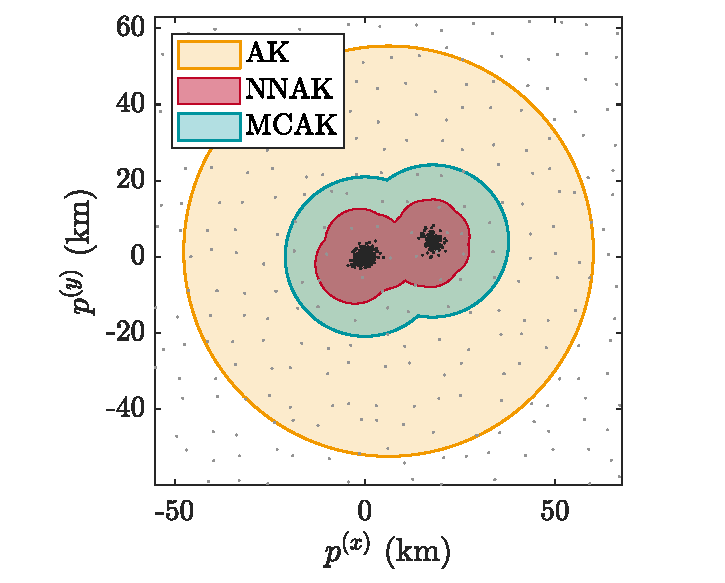
\includegraphics[width=0.7\textwidth]{../../Images/Formes des fenetres.pdf}
	\caption{}\label{fig:subsampling_windows}
\end{figure}

\begin{figure}[!p]
	\centering
	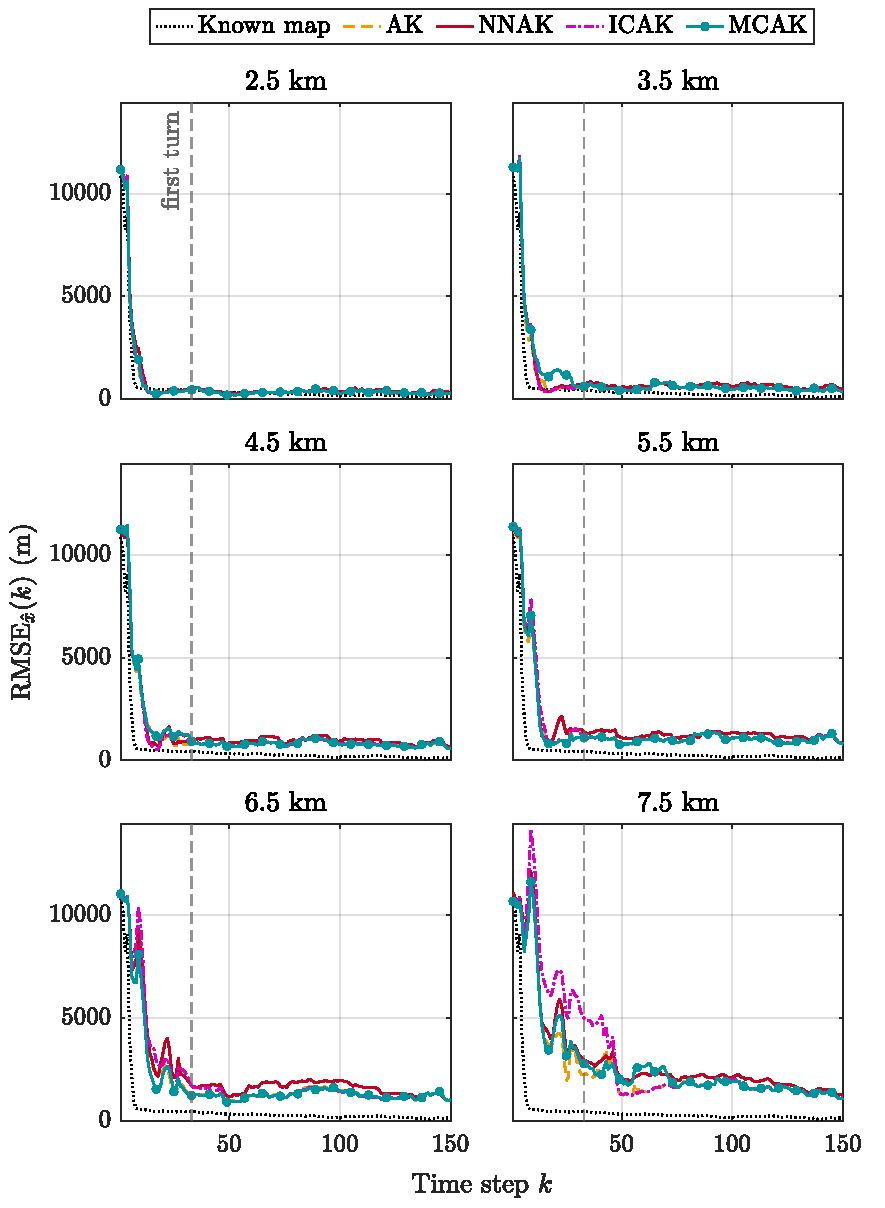
\includegraphics[width=\textwidth]{../../Images/RMSE fenetres par maille.pdf}
	\caption{}\label{fig:fenetres_RMSE}
\end{figure}

\begin{figure}[!p]
	\centering
	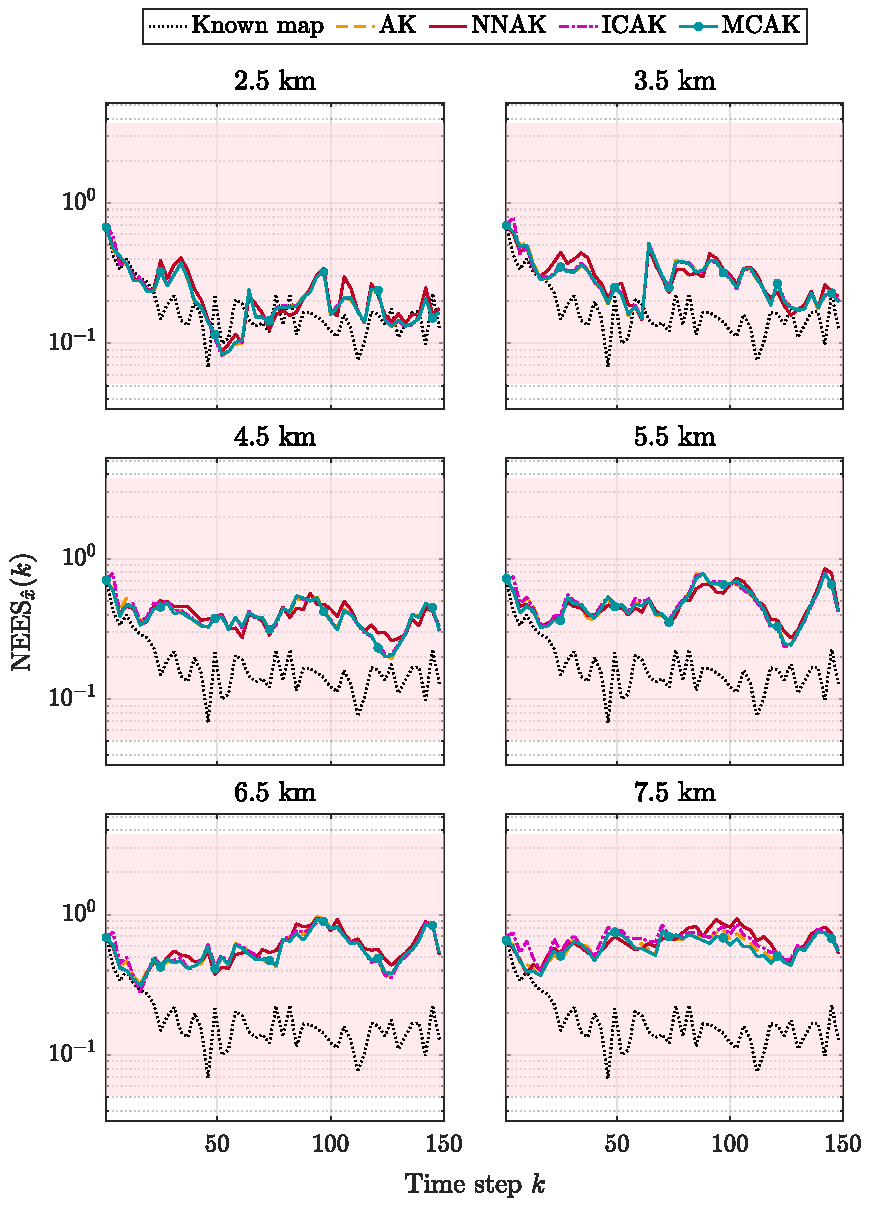
\includegraphics[width=\textwidth]{../../Images/NEES fenetres par maille.pdf}
	\caption{}\label{fig:fenetres_NEES}
\end{figure}

\begin{figure}[!htb]
	\centering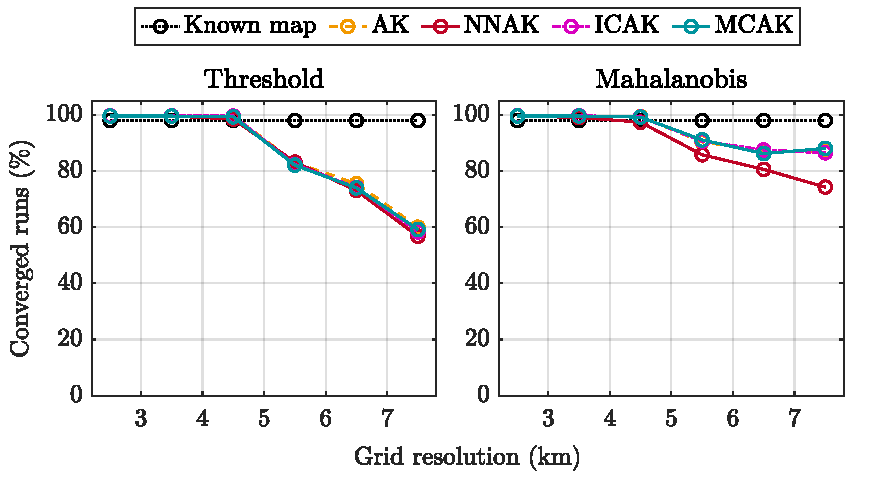
\includegraphics[width=\textwidth]{../../Images/Convergence fenetres.pdf}
	\caption{}\label{fig:convergence_fenetres}
\end{figure}

\begin{table}[!htb]
	\centering% Generated by figures_campagnes.m, do not edit by hand.
% AK against NNAK, ICAK and MCAK.
% Analytic flop counts per run, not timings, for 5000 particles over 150 steps.
% The kriging column gathers the factorisation and the queries, which no
% method pays one without the other; the hyperparameter column is the local
% fits, and the last column, where there is one, the mean-shift of the ICAK and
% the MCAK, or
% the neighbour search of the NNAK. A method that does not pay a cost has no
% column for it.
% Two headings are abbreviated here, HP for the hyperparameter fits
% and NN for the neighbour search.
% The methods are split over two stacked tables, too many columns for
% one; both carry the same grid resolutions.
% Where the training set is fixed, n^3/3 for the setup plus N n^2 per query.

{\setlength{\tabcolsep}{3pt}%
\begin{tabular}{|c|cc|ccc|}\hline
\multirow{2}{*}{$\Delta_g$} & \multicolumn{2}{c|}{AK} & \multicolumn{3}{c|}{NNAK}\\\cline{2-3}\cline{4-6}
 & Kriging & HP & Kriging & HP & NN\\\hline
$2.5$km & $46$ G & $564$ M & $4.3$ G & $57$ M & $47.3$ M\\
$3.5$km & $14.4$ G & $224$ M & $2.05$ G & $36.1$ M & $43.6$ M\\
$4.5$km & $5.75$ G & $121$ M & $1.23$ G & $25.9$ M & $40.9$ M\\
$5.5$km & $3.09$ G & $89.8$ M & $885$ M & $21.7$ M & $38.8$ M\\
$6.5$km & $1.93$ G & $70.1$ M & $705$ M & $19.4$ M & $36.8$ M\\
$7.5$km & $1.54$ G & $66.7$ M & $603$ M & $18.1$ M & $35.3$ M\\
\hline
\end{tabular}
}

\par\vspace{1ex}
{\setlength{\tabcolsep}{3pt}%
\begin{tabular}{|c|ccc|ccc|}\hline
\multirow{2}{*}{$\Delta_g$} & \multicolumn{3}{c|}{ICAK} & \multicolumn{3}{c|}{MCAK}\\\cline{2-4}\cline{5-7}
 & Kriging & HP & Clustering & Kriging & HP & Clustering\\\hline
$2.5$km & $2.26$ G & $87.3$ M & $114$ M & $2.47$ G & $25.3$ M & $114$ M\\
$3.5$km & $901$ M & $83.2$ M & $158$ M & $811$ M & $21.5$ M & $158$ M\\
$4.5$km & $616$ M & $83.3$ M & $194$ M & $496$ M & $17.2$ M & $195$ M\\
$5.5$km & $547$ M & $91.4$ M & $223$ M & $352$ M & $11.9$ M & $224$ M\\
$6.5$km & $513$ M & $107$ M & $251$ M & $241$ M & $7.12$ M & $253$ M\\
$7.5$km & $499$ M & $131$ M & $270$ M & $150$ M & $3.4$ M & $274$ M\\
\hline
\end{tabular}
}

	\caption{}\label{tab:cout_fenetres}
\end{table}
